\documentclass[12pt,oneside]{uhthesis}
\usepackage{subfigure}
\usepackage[ruled,lined,linesnumbered,titlenumbered,algochapter,onelanguage]{algorithm2e}
\usepackage[spanish]{babel}
\usepackage{amsmath}
\usepackage{amssymb}
\usepackage{amsbsy}
\usepackage{caption,booktabs}
\captionsetup{ justification = centering }
%\usepackage{mathpazo}
\usepackage{float}
\setlength{\marginparwidth}{2cm}
\usepackage{todonotes}
\usepackage{listings}
\usepackage[table]{xcolor}
%\usepackage{multicol}
\usepackage{graphicx}
\floatstyle{plaintop}
%\restylefloat{table}


\usepackage{subfigure}

\usepackage{hyperref}
\usepackage[utf8]{inputenc}

\addbibresource{Bibliography.bib}
% \setlength{\parskip}{\baselineskip}%
\renewcommand{\tablename}{Tabla}
\renewcommand{\listalgorithmcfname}{Índice de Algoritmos}
%\dontprintsemicolon
\SetAlgoNoEnd

\definecolor{codegreen}{rgb}{0,0.6,0}
\definecolor{codegray}{rgb}{0.5,0.5,0.5}
\definecolor{codepurple}{rgb}{0.58,0,0.82}
\definecolor{backcolour}{rgb}{0.95,0.95,0.92}

\lstdefinestyle{mystyle}{
    backgroundcolor=\color{backcolour},   
    commentstyle=\color{codegreen},
    keywordstyle=\color{purple},
    numberstyle=\tiny\color{codegray},
    stringstyle=\color{codepurple},
    basicstyle=\ttfamily\footnotesize,
    breakatwhitespace=false,         
    breaklines=true,                 
    captionpos=b,                    
    keepspaces=true,                 
    numbers=left,                    
    numbersep=5pt,                  
    showspaces=false,                
    showstringspaces=false,
    showtabs=false,                  
    tabsize=4
}

\lstset{style=mystyle}

\title{An\'alisis de rendimiento {\vspace{-0.4 cm}}\\ en \\{\vspace{0.1 cm}} Hyperledger Fabric}
\author{\\\vspace{0.25cm}Bryan Mach\'in Garc\'ia}
\advisor{\\\vspace{0.25cm} MsC. Camilo Denis Gonz\'alez\\\vspace{0.2cm} DrC. Carlos Miguel Leg\'on}
\degree{Licenciado en Ciencia de la Computación}
\faculty{Facultad de Matemática y Computación}
\date{\today \\\vspace{0.25cm}\href{https://github.com/username/repo}{github.com/BryanMachin/Optimal-parameters-for-blockchain-networks-by-Hyperledger-Fabric}}
\logo{Graphics/uhlogo}
\makenomenclature

\renewcommand{\vec}[1]{\boldsymbol{#1}}
\newcommand{\diff}[1]{\ensuremath{\mathrm{d}#1}}
\newcommand{\me}[1]{\mathrm{e}^{#1}}
\newcommand{\pf}{\mathfrak{p}}
\newcommand{\qf}{\mathfrak{q}}
\newcommand{\kf}{\mathfrak{k}}
\newcommand{\kt}{\mathtt{k}}
\newcommand{\mf}{\mathfrak{m}}
\newcommand{\hf}{\mathfrak{h}}
\newcommand{\fac}{\mathrm{fac}}
\newcommand{\maxx}[1]{\max\left\{ #1 \right\} }
\newcommand{\minn}[1]{\min\left\{ #1 \right\} }
\newcommand{\lldpcf}{1.25}
\newcommand{\nnorm}[1]{\left\lvert #1 \right\rvert }
\renewcommand{\lstlistingname}{Ejemplo de código}
\renewcommand{\lstlistlistingname}{Ejemplos de código}



\begin{document}

\frontmatter
\maketitle

\begin{dedication}
    Este trabajo se lo dedicado en especial a mis padres Alberto Mach\'in Santos y Marisela García P\'erez, por su apoyo incondicional y la Fe inquebrantable que siempre han depositado en m\'i. Son una parte importante de mis logros y una motivaci\'on para seguir esforz\'andome. Desde peque\~no me encaminaron hacia una formaci\'on de excelencia.
\end{dedication}
\begin{acknowledgements}
    Agradecimientos
\end{acknowledgements}
\begin{opinion}
El trabajo de diploma \emph{An\'alisis de rendimiento en Hyperledger Fabric} del estudiante Bryan Mach\'in Garc\'ia para optar por el t\'itulo de Licenciado en Ciencia de la Computaci\'on, es un tema de investigaci\'on de suma importancia para el Instituto de Criptograf\'ia porque permite mejorar la eficiencia de los servicios basados en redes \emph{blockchain} de Hyperledger Fabric.\\

El diplomante ha mostrado inter\'es por la investigaci\'on, ha sido receptivo a las sugerencias, cr\'iticas y opiniones de ambos tutores; ganando en conocimiento, dominio del tema, y habilidades para reajustar sus experimentos y presentar resultados.\\
 
Puedo afirmar que ha mostrado disciplina y dedicaci\'on en la realizaci\'on de las tareas, tanto en la redacci\'on del trabajo de diploma, como en la organizaci\'on e investigaci\'on del tema, lo cual se ve reflejado en los resultados entregados por el diplomante. Para ello, comenz\'o con la asimilaci\'on y estudio de las tecnolog\'ias indicadas por los tutores, mostrando adem\'as buenas capacidades de asimilaci\'on e independencia.\\

En consecuencia, se define que la tesis cumple con el rigor metodol\'ogico, cient\'ifico y est\'a en funci\'on de los requisitos definidos, partiendo adem\'as del estudio de fuentes y publicaciones recientes relacionadas al tema de investigaci\'on.\\

Por tanto, hago constar que la tesis re\'une los est\'andares metodol\'ogicos exigidos por la Facultad de Matem\'atica y Computaci\'on de la Universidad de la Habana, para ser presentada y sometida a evaluaci\'on en su ejercicio de defensa.\\

Felicito al diplomante por haber respondido con responsabilidad al desaf\'io del estudio y haber finalizado exitosamente su trabajo de diploma.\\

MsC. Camilo Denis González
\end{opinion}
\begin{resumen}
	Resumen en español
\end{resumen}

\begin{abstract}
	Resumen en inglés
\end{abstract}
\tableofcontents
\setcounter{tocdepth}{3}

%\listoffigures
% \listoftables
% \listofalgorithms
%\lstlistoflistings

\mainmatter

\chapter*{Introducción}\label{chapter:introduction}
\addcontentsline{toc}{chapter}{Introducción}


En 2009 Satoshi Nakamoto introduce Bitcoin [\cite{nakamoto2008bitcoin}], la primera criptomoneda descentralizada. Las criptomonedas fueron las primeras aplicaciones que emplearon la tecnolog\'ia blockchain. Con el tiempo, su aplicaci\'on se ha ramificado a distintas esferas, tales como: salud, cadenas de suministro, sistemas electorales, entre otras [\cite{tama2017critical}]. Cuando se trata de almacenar y compartir datos entre diferentes entidades, la base de datos centralizada tiene algunas limitaciones de notoria importancia para mantener la integridad de sus datos. Una de ellas es su \'unico punto de falla; si hay un ataque, todo el sistema puede fallar. Adem\'as, por motivos de privacidad, pudiera no ser aceptable almacenar los datos en un tercero [\cite{xu2017taxonomy}]. Una posible soluci\'on es elegir una entidad de confianza para almacenar los datos. Sin embargo, dado que estas entidades tienen pol\'iticas diferentes, ser\'ia de mayor complejidad lograr un acuerdo sobre la entidad que almacenar\'a los datos. Por su naturaleza distribuida, blockchain supera estas limitaciones al no existir una autoridad centralizada; cada entidad puede tener una copia de los datos, y todas las entidades deben acordar las transacciones antes de su escritura en la blockchain. Cada bloque de transacciones se refiere al bloque anterior por su \emph{hash}, lo que garantiza la integridad de los datos. Si un atacante intenta modificar cualquier bloque, el cambio se propagar\'a a trav\'es de la cadena y ser\'a reconocido.

En la literatura, existen principalmente dos tipos de blockchains: permisionadas y no permisionadas. El objetivo principal de esta \'ultima es proporcionar accesibilidad p\'ublica y transacciones transparentes, por lo tanto, elimina la confidencialidad. La blockchain permisionada surgi\'o para solucionar el problema de almacenar datos confidenciales, por ejemplo, para aplicaciones m\'edicas. Permite compartir datos y acceder a entidades/usuarios de confianza espec\'ificos [\cite{xu2017taxonomy}]. Sin embargo, estas entidades tienen que obtener un consenso entre ellas para identificar cualquier manipulaci\'on no autorizada de datos. En Bitcoin, se utiliza un esquema de consenso \emph{PoW}, prueba de trabajo, en el que los mineros compiten para resolver un rompecabezas computacionalmente intensivo y una vez que un minero lo resuelve, transmite el nuevo bloque. Una de sus limitaciones es la vulnerabilidad al ataque del 51$\%$ que permite tomar el control de toda la red [\cite{narayanan2016bitcoin}], lo que sucede si una sola entidad posee m\'as del 51$\%$ del poder computacional de la blockchain. En el caso de Peercoin [\cite{king2012ppcoin}] emplea \emph{PoS}, prueba de participaci\'on, para disminuir la sobrecarga computacional de \emph{PoW}. La prueba de participaci\'on se basa en la cantidad de moneda reservada y el tiempo de participaci\'on en la red, pero pueden definirse otros criterios; que una vez establecidos, se inicia el proceso de selecci\'on de nodos de forma aleatoria para validar transacciones o crear nuevos bloques. A diferencia de \emph{PoW}, este enfoque no consume gran cantidad de recursos. Adem\'as, no es vulnerable al ataque del 51$\%$, ya que el atacante necesita poseer m\'as monedas que el resto de la red; causando un aumento en el precio de la moneda, lo que hace que los ataques sean muy costosos. La prueba de trabajo y la prueba de participaci\'on son dos de las t\'ecnicas de consenso que garantizan confianza m\'as comunes en las blockchains no permisionadas, sin importar que el proceso de miner\'ia consuma mucho tiempo. Por el contrario, las blockchains permisionadas emplean protocolos m\'as r\'apidos para lograr el consenso. Entre las plataformas m\'as comunes est\'an Ethereum [\cite{antonopoulos2018mastering}] y Hyperledger Fabric. Ethereum se estableci\'o en 2015 y finalmente se convirti\'o en uno de los marcos de blockchains programables m\'as populares. Si bien Ethereum es m\'as liviano y m\'as f\'acil de usar, no es altamente personalizable. A diferencia, Hyperledger Fabric ha dado pasos sustanciales en virtud de lograr un sistema lo m\'as adaptable posible que garantice un mejor rendimiento para los distintos casos de uso [\cite{valenta2017comparison}], principalmente en ecosistemas empresariales.


\section{Situaci\'on probl\'emica}
Cuando se trata de configuraciones, Hyperledger Fabric brinda un alto grado de libertad a los operadores de red, existen par\'ametros para configurar el rendimiento y latencia de las transacciones que se pueden ajustar para escenarios donde se ejecuten una gran cantidad de transacciones por segundos (\emph{TPS}) o donde ocurra todo lo contrario, y es en dependencia de la configuraci\'on de estos par\'ametros que se puede mejorar el rendimiento de redes blockchain usando Hyperledger Fabric. 
Por lo que el problema consiste en definir un escenario de bajo n\'umero de transacciones por segundos y otro que cuente con un elevado n\'umero de transacciones por segundos; y determinar una configuraci\'on en el canal de comunicaci\'on donde se desarrollan las transacciones, para cada escenario, que posibilite un elevado rendimiento.

\section{Motivaci\'on}
La tecnolog\'ia Blockchain ha brindado un nuevo paradigma para generar confianza en los datos, dentro de un ambiente no necesariamente confiable. Los mecanismos para lograrlo, expuestos hoy en d\'ia, consumen diversos recursos, que en escenarios de gran trasiego de informaci\'on pueden fracturar el correcto funcionamiento de la tecnolog\'ia. Esto nos motiva a realizar un estudio que posibilite minimizar el uso de los recursos siempre y cuando se logre un desempe\~no \'optimo. En el caso de Hyperledger Fabric ha salido a la vanguardia en cuanto a la variedad de opciones configurables que ofrece, por esto amerita el centro de nuestra investigaci\'on.


\section{Objetivos}
\subsection{Objetivo General}
Determinar configuraciones \'optimas para canales de redes blockchain de Hyperledger Fabric en escenarios de mayor o menor volumen de transacciones.

{\vspace{0.5 cm}}

\subsection{Objetivos Espec\'ificos}
\begin{itemize}
\item Configurar y Desplegar una red blockchain de Hyperledger Fabric para cada escenario expuesto.
\item Medir el rendimiento de las redes desplegadas.
\item Analizar los reportes de rendimiento.
\item Determinar los par\'ametros de configuraci\'on \'optimos para cada escenario basado en el an\'alisis de los reportes de rendimento.
\end{itemize}


\chapter{Estado del Arte de la plataforma blockchain Hyperledger Fabric}\label{chapter:state-of-the-art}

Hyperledger Fabric es una de las plataformas blockchain m\'as populares, administrada por Linux Foundation. Se basa en una plataforma privada donde solo los usuarios autenticados participan en ella. Difiere de las plataformas blockchain p\'ublicas que posibilitan la uni\'on de cualquier usuario a la red. Adem\'as, Fabric presenta una arquitectura de ejecuci\'on, orden y validaci\'on que supera los l\'imites de la arquitectura de orden y ejecuci\'on anterior []. Esto mejora sustancialmente la escalabilidad de rendimiento en redes blockchain con un n\'umero elevado de Peers, lo que permite a Fabric ser competente en Global Trade Digitalization [], SecureKey [] y Everledger [].Constituye la primera plataforma blockchain que admite contratos inteligentes creados en lenguajes de programaci\'on de uso general como Java, Golang y Node.js; siendo factible para la mayor\'ia de las empresas en el desarrollo de los contratos inteligentes, sin necesidad de capacidad adicional para aprender lenguajes espec\'ificos de dominio restringidos, conocidos por sus siglas DSL. 

Fabric es compatible con protocolos de consenso conectables que permiten a la plataforma personalizarse de manera eficaz de acuerdo al caso de uso y modelos de confianza de los entes que la integran. 

\chapter{Marco Teórico}\label{chapter:theoretical_framework}

Hyperledger Fabric [\cite{HF}] es una de las plataformas blockchain m\'as populares administrada por Linux Foundation. Constituye una plataforma permisionada de nodos pares, nodos ordenadores y clientes, que conforman organizaciones. Cada uno de estos elementos posee una identidad criptogr\'afica en la red. Todas las entidades de la red tienen visibilidad a las identidades de todas las organizaciones y pueden verificarlas. Difiere de las plataformas blockchain p\'ublicas que posibilitan la uni\'on de cualquier usuario a la red. Adem\'as, Fabric presenta una arquitectura de ejecuci\'on, orden y validaci\'on que supera los l\'imites de la arquitectura de orden y ejecuci\'on anterior [\cite{androulaki2018hyperledger}]. Esto mejora sustancialmente la escalabilidad de rendimiento en redes blockchain con un n\'umero elevado de nodos pares, lo que permite a Fabric ser competente en \emph{Global Trade Digitalization} [\cite{digitizing-global}], \emph{SecureKey} [\cite{securekey}] y \emph{Everledger} [\cite{everledger}].Constituye la primera plataforma blockchain que admite contratos inteligentes creados en lenguajes de programaci\'on de uso general como Java, Golang y Node.js; siendo factible para la mayor\'ia de las empresas en el desarrollo de los contratos inteligentes, sin necesidad de capacidad adicional para aprender lenguajes espec\'ificos de dominio restringidos, conocidos por sus siglas en ingl\'es \emph{DSL}. 

\section{Principales conceptos de Hyperledger Fabric}

\subsection{Chaincode}
El chaincode [\cite{Chaincode}] es un software que define uno o m\'as activos junto a las instrucciones de la transacci\'on para su modificaci\'on. Es el encargado de exponer la l\'ogica de negocio. Hace cumplir las reglas para leer o modificar los pares \emph{llave-valor} u otra informaci\'on de la base de datos de estado. Las funciones de un chaincode se ejecutan a partir de la base de datos del estado actual del libro mayor y se inician mediante una propuesta de transacci\'on dando como resultado un conjunto de escrituras \emph{llave-valor} que puede ser enviado a la red y aplicado al libro mayor en todos los nodos pares. Se pueden implementar en varios lenguajes de programaci\'on. Actualmente, se admiten Go, Node.js y Java.


\subsection{Contrato inteligente}
Los contratos inteligentes de Hyperledger Fabric constituyen la l\'ogica de negocio. Est\'an escritos en chaincode, que son invocados por una aplicaci\'on externa a la blockchain cuando necesita interactuar con el libro mayor [\cite{SmartContract}].


\subsection{Libro mayor}
El libro mayor o \emph{ledger} es un registro secuencial, a prueba de manipulaciones, de todas las transiciones de estado en Hyperledger Fabric. Las transiciones de estado son el resultado de los llamados del chaincode \emph{(transacciones)} presentadas por los miembros participantes. Cada transacci\'on da lugar a un conjunto de pares \emph{llave-valor} de activos que se registran en el libro mayor en forma de creaci\'on, actualizaci\'on o eliminaci\'on.

El libro mayor est\'a compuesto por una cadena de bloques para almacenar el registro inmutable y secuenciado en bloques, as\'i como una base de datos de estado para mantener el estado actual de Fabric. Existe un libro mayor por cada canal. Cada nodo par mantiene una copia del libro mayor para cada canal del que es miembro.

\subsection{Pol\'itica de aprobaci\'on}
Los chaincodes est\'an escritos en lenguajes de prop\'osito general que se ejecutan en nodos pares no confiables en la red. Por tanto, surgen m\'ultiples problemas, uno de car\'acter no determinista, ejecuci\'on, y el otro de confiar en los resultados de cualquier nodo par. La pol\'itica de aprobaci\'on aborda estas dos preocupaciones especificando como parte de una pol\'itica de aprobaci\'on, el conjunto de nodos pares que necesitan simular la transacci\'on y aprobar o firmar digitalmente los resultados de la ejecuci\'on.

\subsection{Protocolo de consenso}
En muchas plataformas Blockchain, no permisionadas, como Ethereum y Bitcoin, cualquier nodo puede participar en el proceso de consenso. Estos sistemas se basan en algoritmos de consenso probabil\'isticos que eventualmente garantizan la consistencia del libro mayor en un alto grado de probabilidad, pero que a\'un son vulnerables a ledgers divergentes, conocidos como \emph{bifurcaci\'on} de ledgers), donde diferentes participantes en la red no comparten la misma visi\'on del orden de transacciones aceptado. 
Hyperledger Fabric funciona de manera diferente. Cuenta con un nodo llamado ordenador que realiza la ordenaci\'on de transacciones, junto con otros nodos ordenadores conformando un servicio de ordenaci\'on. Se basa en un dise\~no de consenso determinista, que garantiza para cualquier bloque validado por un nodo par sea final y correcto.
Entre los protocolos de consenso con que cuenta Fabric en la actualidad est\'an:
\begin{itemize}
\item Raft: Se introdujo a partir de v1.4.1. Es un servicio de ordenaci\'on tolerante a fallas \emph{CFT} basado en una implementaci\'on del protocolo Raft en \emph{etcd}\footnote{almacena un conjunto de \emph{llave-valor} distribuido y consistente que proporciona una forma confiable de almacenar datos. Maneja con eficacia las elecciones de l\'ider durante las particiones de la red y puede tolerar fallas, incluso en el nodo l\'ider.}. Sigue un modelo de "l\'ider y seguidor", donde se elige un nodo l\'ider (por canal) y sus decisiones son replicadas por los seguidores. Su dise\~no permite que diferentes organizaciones contribuyan con nodos a un servicio de ordenaci\'on distribuido.

\item Kafka: Similar a Raft, Apache Kafka es una implementaci\'on de \emph{CFT} que utiliza un nodo de "l\'ider y seguidor". Utiliza un conjunto \emph{Zookeeper} [\cite{junqueira2013zookeeper}] con fines de gesti\'on. El consenso basado en Kafka ha estado disponible desde Fabric v1.0, pero muchos usuarios pueden encontrar que administrar un cl\'uster de Kafka es poco deseable.

\item Solo: La implementaci\'on del servicio de ordenaci\'on de \emph{Solo} est\'a destinada solo a prueba, y consiste en un \'unico nodo ordenador.
\end{itemize}

\subsection{Sistema de chaincode}
Un sistema de chaincode tiene el mismo modelo de programaci\'on que los chaincodes de usuarios, pero est\'a integrado en el ejecutable del nodo par. Fabric implementa varios sistemas de chaincodes:
\begin{itemize}
\item Sistema de chaincode de ciclo de vida \emph{(LSCC)}: Permite instalar/crear instancias/actualizar chaincodes.

\item Sistema de chaincode de respaldo \emph{(ESCC)}: Permite aprobar una transacci\'on firmando digitalmente la respuesta.

\item Sistema chaincode de validaci\'on \emph{(VSCC)}: Posibilita evaluar la aprobaci\'on en la transacci\'on contra la pol\'itica de aprobaci\'on especificada para el chaincode. Si la pol\'itica de aprobaci\'on no se satisface, entonces la transacci\'on se toma como inv\'alida.

\item Control de Multiversi\'on de concurrencia [\cite{papadimitriou1984concurrency}] \emph{MVCC}: Garantiza que las versiones de las llaves le\'idas por una transacci\'on durante la fase de aprobaci\'on son igual que su estado actual en el libro mayor local en la fase de confirmaci\'on. Se asemeja a una verificaci\'on de conflicto de lectura y escritura realizada para el control de concurrencia, y se realiza secuencialmente en todas las transacciones v\'alidas en el bloque. Si las versiones del conjunto de lectura no coinciden, denota que anteriormente la transacci\'on modific\'o los datos le\'idos y fue desde su aprobaci\'on confirmada con \'exito, la transacci\'on es designada como inv\'alida. Para garantizar que no se produzcan lecturas fantasmas la consulta se vuelve a ejecutar y se comparan los \emph{hashes} de los resultados, que tambi\'en se almacena como parte del conjunto de lectura, capturado durante la aprobaci\'on.

\item Sistema de configuraci\'on chaincode \emph{(CSCC)}: Permite administrar las configuraciones de los canales.
\end{itemize}


\subsection{Canal}
Hyperledger Fabric introduce un concepto llamado \emph{canal} como una subred privada de comunicaci\'on entre dos o m\'as nodos pares para proporcionar un nivel de aislamiento. Las transacciones en un canal solo son vistos por sus nodos pares y participantes. El ledger y los chaincodes son definidos por canal. Adem\'as, el consenso es aplicable por canal, es decir, no hay un orden definido para la transacci\'on a trav\'es de los canales.

\subsection{Servicio de membres\'ia}
El servicio de membres\'ia o proveedor de servicios de membres\'ia \emph{MSP} [\cite{MSP}] es un conjunto de carpetas que se agregan a la configuraci\'on de la red y se emplea para definir una organizaci\'on, tanto interna, como externamente. Mientras que las autoridades de certificaci\'on (\emph{CA}) generan los certificados que representan a cada identidad, el \emph{MSP} contiene una lista de identidades autorizadas.

El \emph{MSP} identifica la autoridad certificadora ra\'iz, y las intermedias se aceptan para definir los miembros de un dominio de confianza enumerando las identidades de sus miembros o identificando qu\'e \emph{CA} est\'an autorizadas para emitir identidades v\'alidas para sus miembros.

El poder de un \emph{MSP} va m\'as all\'a de enumerar qui\'en es un participante de la red o miembro de un canal. Convierte una identidad en un rol al identificar los privilegios espec\'ificos que tiene un actor en un nodo o canal. Cuando un usuario est\'a registrado con \emph{Fabric CA}, se debe asociar con el usuario una funci\'on de administrador, nodo par, cliente, nodo ordenador o miembro.\\ 


Los \emph{MSP} coexisten en dos dominios dentro de la blockchain:
\begin{itemize}
\item Servicio de membres\'ia local: Se define para clientes y nodos (pares y ordenadores). Los \emph{MSP} locales definen los permisos para un nodo. Los \emph{MSP} locales de los clientes permiten al usuario autenticarse en sus transacciones como miembro de un canal, por ejemplo, en las transacciones, o como propietario de un rol espec\'ifico en el sistema.

\item Servicio de membres\'ia del canal: Define los derechos administrativos y de participaci\'on a nivel de canal. Los nodos pares y los nodos ordenadores en un canal de aplicaci\'on comparten la misma vista de los \emph{MSP} del canal y, por lo tanto, pueden autenticar correctamente a los participantes del canal. Esto significa que, si una organizaci\'on desea unirse al canal, se debe incluir en la configuraci\'on del canal un \emph{MSP} que incorpore la cadena de confianza para los miembros de la organizaci\'on. De lo contrario, se rechazar\'an las transacciones que se originen a partir de las identidades de esta organizaci\'on. Mientras que los \emph{MSP} locales se representan como una estructura de carpetas en el sistema de archivos, los \emph{MSP} de canal se describen en una configuraci\'on de canal.
\end{itemize}

\subsection{Autoridad certificadora}
Un nodo puede participar en la red blockchain, a trav\'es de una identidad digital emitida por una autoridad de confianza del sistema. Las identidades digitales constituyen certificados digitales validados criptogr\'aficamente que cumplen con el est\'andar X.509 y son emitidos por una Autoridad de Certificaci\'on(\emph{CA}) [\cite{CA}]. Las \emph{CA} tienen un certificado, que ponen a disposici\'on de todos para que los consumidores de identidades emitidas por una determinada \emph{CA} verifiquen comprobando que el certificado s\'olo pudo haber sido generado por el titular de la clave privada correspondiente.

\subsubsection{Fabric CA}
Fabric proporciona un componente de \emph{CA} que permite crear identidades en la red blockchain. Es un proveedor de \emph{CA} ra\'iz privado capaz de administrar las identidades digitales de los participantes de Fabric que tienen la forma de certificados X.509. Debido a que \emph{Fabric CA} es una \emph{CA} personalizada dirigida a las necesidades de \emph{CA} ra\'iz de Fabric, no es capaz de proporcionar certificados \emph{SSL} para uso general en navegadores. Sin embargo, debido a que se debe usar alguna \emph{CA} para administrar la identidad (incluso en un entorno de prueba), \emph{Fabric CA} se puede usar para proporcionar y administrar certificados. Tambi\'en es posible, utilizar una \emph{CA} ra\'iz p\'ublica/comercial o intermedia para proporcionar identificaci\'on.

\subsection{Nodo Par}
Un nodo par ejecuta el chaincode, que implementa un contrato inteligente del usuario y mantiene el ledger en un sistema de archivos. El chaincode tiene acceso permitido al estado compartido definido por la \emph{API}. Entre los nodos pares se distinguen los que mantienen la l\'ogica del chaincode y lo ejecuta para aprobar una transacci\'on. Sin tener en consideraci\'on esta diferenciaci\'on, todos mantienen el libro mayor y el \'ultimo estado \emph{StateDB} en un registro de \emph{llave-valor} tal que se puede consultar o modificar el estado.

\subsection{Nodo Ordenador}
Los nodo ordenador participa en el protocolo de consenso y conforma el bloque de transacciones que se entrega a los nodos pares mediante un protocolo de comunicaci\'on \emph{gossip}\footnote{El protocolo \emph{Gossip} es un protocolo que permite dise\~nar sistemas de comunicaciones distribuidos (\emph{P2P}) altamente eficientes, seguros y de baja latencia.}. Juntos constituyen el servicio de ordenaci\'on, \emph{OSN} por sus siglas en ingl\'es, que posee un car\'acter modular y admite un mecanismo de consenso \emph{conectable}. Se construye un bloque para ser entregado a los nodos pares, cuando se llega a un n\'umero m\'aximo de nuevas transacciones desde el \'ultimo bloque conformado, o se cumple al tiempo de espera configurado desde la \'ultima transacci\'on producida.

\subsection{Cliente}
Los clientes son responsables de llevar a cabo una propuesta de transacci\'on a uno o m\'as nodos pares simult\'aneamente para recopilar respuestas a propuestas y satisfacer la pol\'itica de aprobaci\'on. Posteriormente transmiten la transacci\'on al servicio de ordenaci\'on para ser incluida en un bloque y entregado a todos los pares para su validaci\'on y confirmaci\'on.

\section{Flujo de transacciones en Hyperledger Fabric}
A diferencia de otras redes Blockchain que emplean un modelo de \emph{ordenaci\'on-ejecución} [\cite{vukolic2017rethinking}] de transacciones, Fabric emplea un modelo de simulaci\'on, validaci\'on y confirmaci\'on de transacciones.\\ 

La figura \ref{FlujoTransacciones} muestra el flujo de la transacci\'on que consta de 3 fases:
\begin{itemize}
\item[1] Fase de aprobaci\'on: Simula la transacci\'on en nodos pares selectivos y recopila los cambios de estado.
\item[2] Fase de ordenaci\'on: Ordena las transacciones a trav\'es de un protocolo de consenso.
\item[3] Fase de validaci\'on: Valida y confirma en el libro mayor.
\end{itemize}



\begin{figure}[h]
\centering
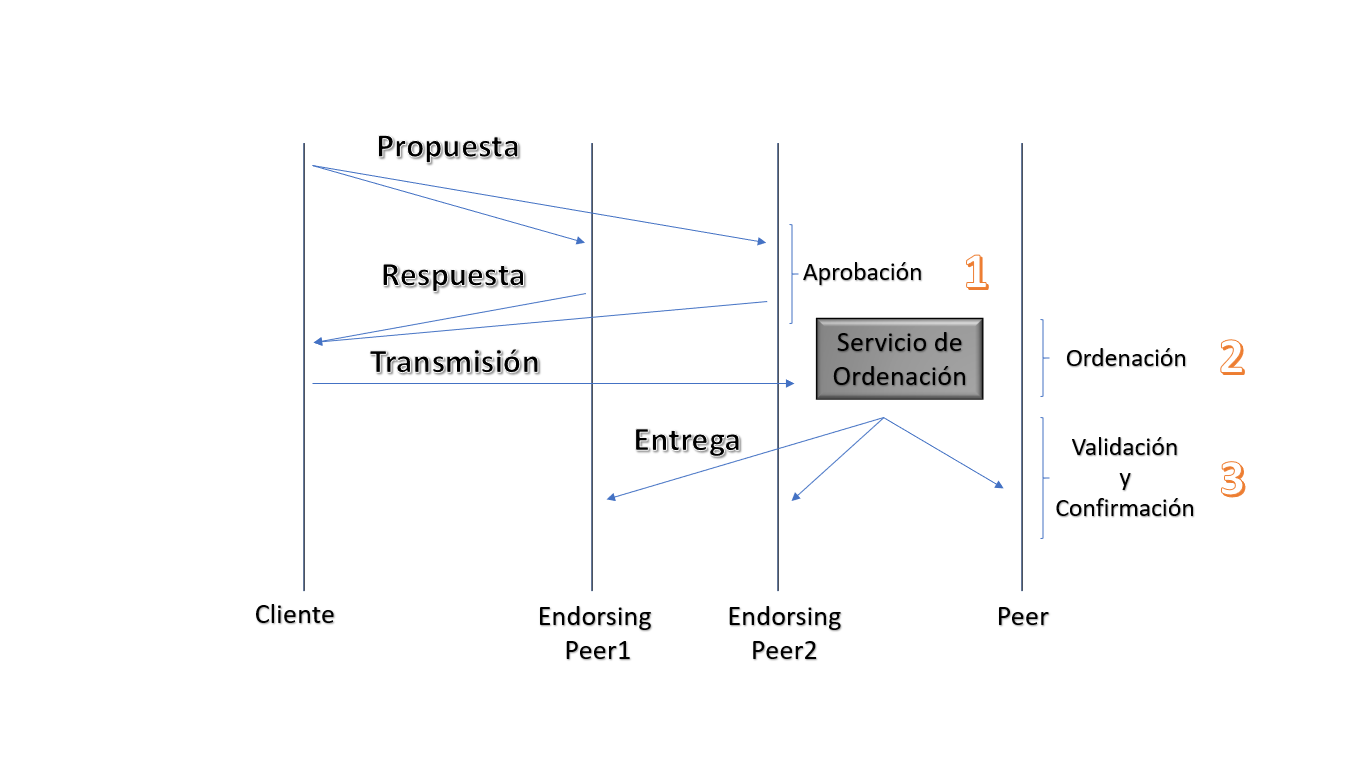
\includegraphics[width=0.6\linewidth]{Graphics/FlujoTransacciones.png}
\caption{Flujo de transacciones.}
\label{FlujoTransacciones}
\end{figure}

\vspace{1 cm}
Antes de que las transacciones sean enviadas, la red debe comenzar con las organizaciones participantes, sus \emph{MSP} e identidades de los nodos pares. Primero, se crea un canal en la red con los respectivos \emph{MSP} de las organizaciones. En segundo lugar, los nodos pares de cada organizaci\'on se unen al canal y se inicializa el libro mayor. Finalmente, los chaincodes requeridos se instalan en el canal.


\subsection{Fase de aprobaci\'on}
Una aplicaci\'on cliente que utiliza Fabric \emph{SDK} [\cite{Go-SDK}], [\cite{Node-SDK}], [\cite{Java-SDK}], construye una propuesta de transacci\'on para invocar un chaincode que a su vez realizar\'a operaciones en el estado del libro mayor. La propuesta est\'a firmada con las credenciales del cliente y el cliente lo env\'ia a uno o m\'as nodos pares simult\'aneamente. La pol\'itica de aprobaci\'on del chaincode dicta los nodos pares de la organizaci\'on que el cliente necesita para enviar la propuesta a la simulaci\'on. 

Primero, cada nodo par que aprueba, verifica que el remitente es autorizado para invocar transacciones en el canal. En segundo lugar, el nodo ejecuta el chaincode, que puede acceder al estado actual del libro mayor en el nodo par. Los resultados de la transacci\'on incluyen el valor de respuesta, conjunto de lectura y conjunto de escritura. En tercer lugar, el par que aprueba llama a un sistema chaincode llamado \emph{ESCC} que firma esta respuesta de transacci\'on con la identidad del nodo par y responde al cliente. Finalmente, el cliente inspecciona la respuesta de la propuesta a verificar que lleva la firma del nodo par. El cliente recoge las respuestas de diferentes nodos pares y verifica que sea la misma. Dado que cada nodo par pod\'ia haber ejecutado la transacci\'on en diferentes momentos en la Blockchain, es posible que la respuesta de la propuesta difiera. En tales casos, el cliente tiene que volver a enviar la propuesta a otros pares, para obtener suficientes respuestas coincidentes.

\subsection{Fase de ordenaci\'on}
El cliente transmite un mensaje de transacci\'on bien formado al servicio de ordenaci\'on. La transacci\'on tendr\'a los conjuntos de lectura y escritura, las firmas de los nodos pares que aprueban y la identificaci\'on del canal. El servicio de ordenaci\'on no necesita inspeccionar el contenido de la transacci\'on para realizar su operaci\'on. Recibe transacciones de diferentes clientes por varios canales y los pone en cola por canal. Crea bloques de transacciones por canal, firma el bloque con su identidad y los entrega a los nodos pares usando el protocolo de mensajer\'ia \emph{gossip}.

\subsection{Fase de validaci\'on}
Todos los nodos pares en un canal reciben bloques de la red. Cada nodo par primero verifica la firma del nodo ordenador en el bloque. Cada bloque v\'alido se decodifica y todas las transacciones en un bloque pasan primero por una validaci\'on de \emph{VSCC} antes de realizar la validaci\'on de \emph{MVCC}.

\subsection{Fase de actualizaci\'on en el libro mayor}
Como \'ultimo paso del procesamiento de transacciones, el libro mayor se actualiza agregando el bloque al libro mayor local \emph{StateDB}, que contiene el estado actual de todas las llaves. Se actualiza con los conjuntos de escritura de transacciones v\'alidas. Estas actualizaciones de \emph{StateDB} se realizan para un bloque de transacciones y aplican las actualizaciones para llevar \emph{StateDB} al estado despu\'es de que se hayan procesado todas las transacciones en el bloque.

\section{Par\'ametros configurables}
Nuestro objetivo es estudiar el rendimiento de Fabric en diversas condiciones para comprender c\'omo las elecciones de las diferentes facetas del sistema afectan el rendimiento. Sin embargo, el espacio de par\'ametros es amplio y limitamos nuestras opciones para cubrir de manera integral algunos componentes y observar ampliamente otros aspectos del sistema para que podamos identificar la interacci\'on de las opciones a nivel de componentes.

\subsection{Tama\~no de bloque}
Las transacciones se procesan por lotes en el nodo ordenador y se entregan como un bloque a los nodos pares usando un protocolo \emph{gossip}. Cada nodo par procesa un bloque a la vez. La variaci\'on del tama\~no de bloque tambi\'en trae consigo la compensaci\'on de rendimiento frente a latencia y, para obtener una mejor concepci\'on, lo estudiamos en conjunto con la tasa de llegada de transacciones.

\subsection{Pol\'itica de aprobaci\'on}
Una pol\'itica de aprobaci\'on dicta cu\'antas ejecuciones de una transacci\'on y firma deben ocurrir antes de que se pueda enviar una solicitud de transacci\'on al servicio de ordenaci\'on para que la transacci\'on pueda pasar la fase de validaci\'on \emph{VSCC} en los pares. La validaci\'on \emph{VSCC} de los aprobados de una transacci\'on requiere la evaluaci\'on de la expresi\'on de la pol\'itica de aprobaci\'on frente a los aprobados recopilados y la verificaci\'on de la satisfacibilidad [\cite{gottlieb2002evolutionary}], que es \emph{NP-Completo}. Adicionalmente, incluye verificar la identidad y su firma. La complejidad de la pol\'itica de aprobaci\'on afectar\'a los recursos y el tiempo necesario para recopilar y evaluar transacciones.

\subsection{Canal}
Los canales a\'islan las transacciones. Las transacciones enviadas a diferentes canales se ordenan, entregan y procesan de forma independiente, aunque en el mismo nodo par. Los canales aportan un paralelismo inherente a varios aspectos de procesamiento de transacciones en Hyperledger Fabric. Mientras que el n\'umero de canales a emplear, y en qu\'e canales realizar transacciones est\'a determinado por la aplicaci\'on y la combinatoria de los participantes, tiene importantes implicaciones en el rendimiento y la escalabilidad de la plataforma.

\subsection{Recursos}
Los nodos pares ejecutan la firma y verificaci\'on como parte de un sistema chaincode con empleo intensivo de la \emph{CPU}.

\subsection{Base de datos del libro mayor}
Fabric admite dos alternativas para almacenar \emph{llave-valor}, \emph{CouchDB} [\cite{CouchDB}] y \emph{GoLevelDB} [\cite{GoLevelDB}] para mantener el estado actual. Ambos almacenan \emph{llave-valor}, mientras que \emph{GoLevelDB} es una base de datos incrustada, \emph{CouchDB} usa un modelo \emph{cliente-servidor} (al que se accede mediante la \emph{API REST} a trav\'es de un \emph{HTTPS}) y es compatible con documentos \emph{JSON}.

\section{Hyperledger Fabric v2.x}
La primera versi\'on de notoria importancia de Hyperledger Fabric luego de su lanzamiento con la versi\'on 1.0 fue Fabric v2.0. Ofrece nuevas caracter\'isticas y cambios representativos para usuarios y operadores [\cite{NewHF}]. Incluye la compatibilidad con nuevos patrones de aplicaciones y privacidad, gobernanza mejorada en torno a contratos inteligentes y nuevas opciones para nodos operativos.\\

Fabric v2.0 presenta un gobierno descentralizado para contratos inteligentes, con un nuevo proceso para instalar un chaincode en sus nodos pares e instanciarlos en un canal. El nuevo ciclo de vida del chaincode de Fabric permite que varias organizaciones lleguen a un acuerdo sobre los par\'ametros del chaincode, como la pol\'itica de aprobaci\'on del contrato, antes de que pueda usarse para interactuar con el ledger. El nuevo modelo ofrece varias mejoras con respecto al ciclo de vida anterior [\cite{hyperledger2018hyperledger}]:

{\begin{itemize}
\item {\bf M\'ultiples organizaciones deben aceptar los par\'ametros de un chaincode}. En las versiones de lanzamiento 1.x, una organizaci\'on ten\'ia la capacidad de establecer par\'ametros de un chaincode, como la pol\'itica de aprobaci\'on, para todos los miembros del canal, que solo ten\'ian el poder de negarse a instalar el chaincode, por lo tanto, no participar en transacciones que lo invoquen. El nuevo ciclo de vida del chaincode de Fabric es m\'as flexible, admite tanto el modelo de ciclo de vida anterior, como modelos descentralizados que requieren suficiente n\'umero de organizaciones para acordar una pol\'itica de aprobaci\'on y otros detalles antes de que el chaincode se convierta en activo en un canal.

\item {\bf Proceso de actualizaci\'on de chaincode m\'as deliberado}. Anteriormente la transacci\'on de actualizaci\'on pod\'ia ser emitida por una sola organizaci\'on, creando un riesgo para un miembro del canal que a\'un no hab\'ia instalado el nuevo chaincode. El nuevo modelo permite que el chaincode se actualice solo despu\'es de que un n\'umero suficiente de organizaciones han aprobado la actualizaci\'on.

\item {\bf Actualizaciones m\'as sencillas de pol\'iticas de respaldo y recopilaci\'on de datos privados}. Se permite cambiar una pol\'itica de respaldo o una configuraci\'on de recopilaci\'on de datos privados sin tener que volver a empaquetar o instalar el chaincode. Los usuarios tambi\'en pueden aprovechar una nueva pol\'itica de aprobaci\'on predeterminada que requiere la aprobaci\'on de una mayor\'ia de organizaciones en el canal. Esta pol\'itica se actualiza autom\'aticamente cuando se agregan o eliminan organizaciones del canal.

\item {\bf Paquetes de chaincodes inspeccionables}. El chaincode se empaqueta en archivos {\bf .tar} f\'aciles de leer, que hace m\'as factible su inspecci\'on y coordinaci\'on de la instalaci\'on en m\'ultiples organizaciones.

\item {\bf Iniciar m\'ultiples chaincodes en un canal usando un paquete}. El ciclo de vida anterior defin\'ia cada chaincode en el canal usando un nombre y una versi\'on que se especific\'o en su instalaci\'on. Ahora existe la posibilidad de usar un solo paquete de chaincodes y desplegarlo varias veces con diferentes nombres en el mismo canal o en diferentes canales.

\item {\bf Los paquetes de chaincode no necesitan ser iguales entre los miembros del canal}. Las organizaciones pueden extender un chaincode para su propio caso de uso, por ejemplo, para realizar diferentes validaciones en inter\'es de su organizaci\'on. Siempre que el n\'umero requerido de organizaciones respalde las transacciones del chaincode con resultados coincidentes, la transacci\'on se validar\'a y se confirmar\'a en el libro mayor. Esto tambi\'en permite a las organizaciones implementar arreglos menores individualmente.
\end{itemize}

Los mismos m\'etodos descentralizados para llegar a un acuerdo que sustentan la nueva gesti\'on del ciclo de vida del chaincode pueden usarse tambi\'en en su propia aplicaci\'on para garantizar que las organizaciones den su consentimiento a las transacciones de datos antes de que se realicen escrituras en el libro mayor.\\

\begin{itemize}
\item {\bf Comprobaciones automatizadas}. Las organizaciones pueden agregar comprobaciones autom\'aticas a las funciones del chaincode para validar informaci\'on adicional antes de aprobar una propuesta de transacci\'on.

\item {\bf Acuerdo descentralizado}. Las decisiones humanas se pueden modelar en un proceso de chaincode que abarca m\'ultiples transacciones. El chaincode puede requerir que los actores de varias organizaciones indiquen sus t\'erminos y condiciones de acuerdo en una transacci\'on en el libro mayor. Luego, una propuesta final de chaincode puede verificar que las condiciones de todas las transacciones individuales se cumplen y establecer la transacci\'on comercial con car\'acter definitivo en todos los miembros del canal.
\end{itemize}

Fabric v2.0 tambi\'en permite nuevos patrones para trabajar y compartir datos privados, sin el requisito de crear recopilaciones de datos privados para todas las combinaciones de miembros del canal que deseen realizar transacciones. Espec\'ificamente, en lugar de compartir datos privados dentro de una colecci\'on de varios miembros. Es posible compartir datos privados entre colecciones, donde cada colecci\'on puede incluir una sola organizaci\'on, o tal vez una sola organizaci\'on junto con un regulador o auditor.\\

\begin{itemize}
\item {\bf Compartir y verificar datos privados}. Cuando los datos privados se comparten con un miembro del canal que no es miembro de una colecci\'on, o compartida con otra colecci\'on de datos privados que contiene uno o m\'as miembros del canal (escribiendo una llave para esa colecci\'on), las partes receptoras pueden utilizar la \emph{API} del chaincode \emph{GetPrivateDataHash()} para verificar que los datos privados coincidan con los \emph{hash} en la cadena que se crearon a partir de datos privados en transacciones anteriores.

\item {\bf Pol\'iticas de aprobaci\'on a nivel de colecci\'on}. Las colecciones de datos privados ahora se pueden definir opcionalmente con una pol\'itica de aprobaci\'on que anula la pol\'itica de aprobaci\'on a nivel de chaincode para las llaves dentro de la colecci\'on. Se puede usar para restringir qu\'e organizaciones pueden escribir datos en una colecci\'on. Se puede concebir un chaincode que requiere el respaldo de la mayor\'ia de las organizaciones, pero para cualquier transacci\'on determinada, puede necesitar dos organizaciones transaccionales para respaldar individualmente su acuerdo en sus propias colecciones de datos privados.

\item {\bf Recopilaciones impl\'icitas por organizaci\'on}. Si se desea utilizar patrones de datos privados por organizaci\'on, no se necesita definir las colecciones al implementar chaincode. Las colecciones se pueden usar sin ninguna definici\'on inicial.
\end{itemize}

La funci\'on de lanzador de chaincode externo permite a los operadores crear y lanzar chaincode con la tecnolog\'ia de su elecci\'on. No se requiere el uso de constructores y lanzadores externos ya que el comportamiento predeterminado construye y ejecuta el chaincode de la misma manera que las versiones anteriores con la \emph{API} de Docker.

\begin{itemize}
\item {\bf Elimina la dependencia del demonio de Docker}. Las versiones anteriores de Fabric requer\'ian que los nodos pares tuvieran acceso a un \emph{Docker daemon}  para construir y lanzar chaincode, algo que puede no ser deseable en entornos de producci\'on.

\item {\bf Alternativas a los contenedores}. Ya no es necesario ejecutar chaincode en contenedores Docker, y puede ejecutarse en el entorno elegido por el operador (incluidos los contenedores).


\item {\bf Chaincode como un servicio externo}. Tradicionalmente, los chaincodes son lanzados por el nodo par y luego se conectan de nuevo a \'el. Ahora es posible ejecutar chaincode como un servicio externo, por ejemplo, en un \emph{pod} de Kubernetes, que un nodo par puede conectarse y utilizar para la ejecuci\'on de chaincode.
\end{itemize}

Cuando se utiliza una base de datos de estado externa \emph{CouchDB}, los retrasos de lectura durante las fases de aprobaci\'on y validaci\'on han representado un cuello de botella en el rendimiento. Con Fabric v2.0, una nueva cach\'e reemplaza muchas de estas costosas b\'usquedas con lecturas r\'apidas de cach\'e local. El tama\~no de cach\'e se configura mediante la propiedad \emph{cacheSize} en \emph{core.yaml}.\\

Hyperledger Fabric v2.3 presenta dos nuevas caracter\'isticas para mejorar las operaciones entre los nodos pares y ordenadores:

\begin{itemize}
\item {\bf Gesti\'on de canales de ordenaci\'on sin un canal de sistema}. Para simplificar el proceso de creaci\'on de canales y mejorar la privacidad y escalabilidad de los canales, es posible crear canales de aplicaci\'on sin crear primero un \emph{canal de sistema} administrado por el servicio de ordenaci\'on. Este proceso permite ordenar a los nodos que se unan (o abandonen) cualquier cantidad de canales seg\'un sea necesario.

\item {\bf Copia del libro mayor}. Ahora es posible tomar una copia de la informaci\'on del canal en un par, incluida su base de datos de estado, y unir nuevos pares (en la misma organizaci\'on o en diferentes organizaciones) al canal en funci\'on de la copia.
\end{itemize}

Con las \'ultimas versiones de Fabric v2.4 se introduce \emph{Fabric Gateway} que elimina gran parte del env\'io de transacciones y la l\'ogica de consulta de la aplicaci\'on del cliente y la cambia a una puerta de enlace com\'un que se ejecuta dentro de los nodos pares, lo que permite que cada uno de los \emph{SDK} del cliente sean m\'as ligeros y requieran menos mantenimiento. Las aplicaciones interact\'uan con un nodo par de confianza (por ejemplo, en su organizaci\'on) que coordina la aprobaci\'on de otros nodos pares y el env\'io al servicio de ordenaci\'on. Tambi\'en simplifica la sobrecarga administrativa de ejecutar una red Fabric porque las aplicaciones cliente pueden conectarse y enviar transacciones a trav\'es de un solo puerto de red en su organizaci\'on en lugar de abrir puertos desde una aplicaci\'on cliente a m\'ultiples nodos pares.

Tambi\'en se agrega el comando conocido como \emph{peer unjoin} que permite a un administrador eliminar un nodo par de un canal. El nodo par debe detenerse cuando se ejecuta el comando para que se puedan limpiar los artefactos propios del canal, como: el ledger del canal y la base de datos de estado. Una vez que se reinicia el nodo par, no recibirá nuevos bloques para el canal.

A partir de Fabric v2.4 se puede determinar el ID del paquete de un chaincode sin instalarlo en los nodos pares mediante el nuevo comando de ciclo de vida del nodo par \emph{chaincodecalculatepackageid}. Entre otras virtudes, posibilita verificar si un paquete de chaincode espec\'ifico est\'a instalado o no sin necesidad de instalarlo.
\chapter{Propuesta}\label{chapter:proposal}

La variaci\'on en las configuraciones de Hyperledger Fabric tiene una influencia directa en los tiempos de asimilaci\'on y procesamiento de las transacciones. Se propuso un an\'alisis del comportamiento de varias configuraciones de redes (v\'ease en la tabla \ref{tab:MisConfiguraciones}), donde var\'ian el n\'umero de nodos pares y ordenadores, adem\'as del tama\~no de los bloques en la configuraci\'on del canal al cual pertenecen. Se tomaron como variables de estudio: latencia m\'inima, latencia m\'axima, latencia promedio y el rendimiento de la red, en funci\'on del n\'umero de transacciones procesadas en un segundo. Para evaluar el desempe\~no de los nodos pares, se fij\'o el n\'umero de nodos ordenadores en 1 para evitar sesgos en las mediciones. En el caso de los ordenadores, se fijaron en 2 el n\'umero de nodos pares. Cada nodo par fue configurado para cumplir con la pol\'itica de aprobaci\'on. Las configuraciones se evaluaron, durante 60 segundos, para dos escenarios con un valor fijo de acuerdo al volumen de transacciones: bajo y alto, con 10 y 100 transacciones por segundo respectivamente. Los nodos ordenadores se chequearon durante 30 segundos a un ritmo fijo de 50 TPS. Como factor determinante se estudi\'o la influencia del tama\~no de los bloques en la latencia promedio y el rendimiento. Para esto se evaluaron tres posibles candidatos a tama\~no de bloques: 10, 50 y 100. Para los escenarios de bajo y alto volumen de transacciones se propuso un conjunto de par\'ametros que, de acuerdo a las necesidades, maximizan el rendimiento de las componentes en la red o minimiza la latencia promedio de las transacciones.
\chapter{Detalles de Implementación y Experimentos}\label{chapter:implementation}

El estudio se realiz\'o en un sistema operativo Ubuntu 22.04 LTS con una CPU Intel Core i3-5020U 2.20Ghz y 12GB 1600MHz RAM. Se utiliz\'o Docker 19.03.8 para las im\'agenes de Fabric v2.4.\\

Para configurar la red se utiliz\'o Minifabric en su versi\'on m\'as reciente. Las pruebas de rendimiento se realizaron con Caliper v0.5.0 empleando el \emph{chaincode} \emph{samplecc} suministrado por Minifabric.\\

Los nodos ordenadores emplearon el mecanismo de consenso \emph{raft} en cada una de las configuraciones y los nodos pares, \emph{GoLevelDB} como base de datos de estado. Se destaca el empleo del voto por mayor\'ia en la pol\'itica de aprobaci\'on, donde todos los nodos pares fueron igualmente configurados para participar en ella. Se tuvo en cuenta el estudio en una sola organizaci\'on, pero de acuerdo a la pol\'itica de aprobaci\'on implantada, su comportamiento simula para $n$ nodos pares, una red con $n$ organizaciones de un nodo par cada una, donde se evita el sesgo que propicia la conectividad en las organizaciones y a su vez se tiene un acceso homog\'eneo de los recursos del \emph{hardware}.

\newpage
\section{Escenario de bajo volumen de transacciones}

En las tablas \ref{tab:10TPS-10BS}, \ref{tab:10TPS-50BS} y \ref{tab:10TPS-100BS} se registran los datos obtenidos para el escenario de 10 TPS.\\

\subsection{An\'alisis de latencia}
De acuerdo a los datos suministrados se puede visualizar el comportamiento de las medida de latencia para las configuraciones con diferente tama\~no en los bloques del canal.\\

\begin{figure}[htbp]
\subfigure[Tama\~no de bloque igual 10.]{
\begin{minipage}[t]{0.30\linewidth}
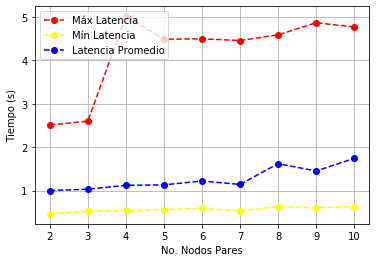
\includegraphics[scale=0.35]{Graphics/AnalisisLatenciaPares10TPSBS10.png}
\end{minipage}
}
\subfigure[Tama\~no de bloque igual 50.]{
\begin{minipage}[t]{0.30\linewidth}
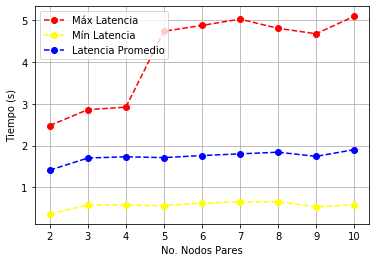
\includegraphics[scale=0.35]{Graphics/AnalisisLatenciaPares10TPSBS50.png}
\end{minipage}
}
\subfigure[Tama\~no de bloque igual 100.]{
\begin{minipage}[t]{0.30\linewidth}
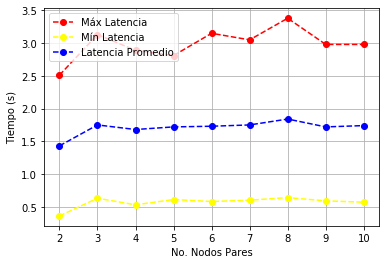
\includegraphics[scale=0.35]{Graphics/AnalisisLatenciaPares10TPSBS100.png}
\end{minipage}
}
\caption{Latencia en distintas configuraciones de nodos pares en una red con un solo nodo ordenador para escenarios de 10 TPS.}
\end{figure}

De acuerdo a la latencia m\'inima, para los tres casos mantienen un comportamiento similar, marcado por una leve tendencia al crecimiento con el aumento del n\'umero de nodos pares en la red. En el caso de la red configurada con un tama\~no de bloque igual a 10, los valores de latencia promedio son m\'as pr\'oximos a los valores de latencia m\'inima con respecto a las dem\'as configuraciones. Esto sucede porque al llegar las transacciones al servicio de ordenaci\'on, como el tama\~no del bloque es menor que el resto, y a su vez tiene una capacidad no superior al n\'umero de transacciones suministradas por los clientes, el tiempo de espera, en promedio, de las transacciones v\'alidas para cerrar el bloque es menor. Esta afirmaci\'on contrasta con la latencia m\'axima que, a menor tama\~no de bloques, mayores valores alcanza producto a que ocurre un proceso de llenado m\'as r\'apido originando una validaci\'on m\'as frecuente en los nodos pares, que a su vez participan en el proceso de simulaci\'on de las transacciones elevando la probabilidad de saturaci\'on en su proceso de ejecuci\'on.\\

En la figura \ref{ComparacionLatencia10TPS} se percibe que para un tama\~no de bloque igual a 10, el valor de latencia promedio es m\'inimo para todos las configuraciones de nodos pares. Luego, el tama\~no de bloque 10 es un par\'ametro que optimiza la latencia promedio en la red, en comparaci\'on a los dem\'as, por tanto, es un posible candidato a \'optimo.\\

\begin{figure}[h]
\centering
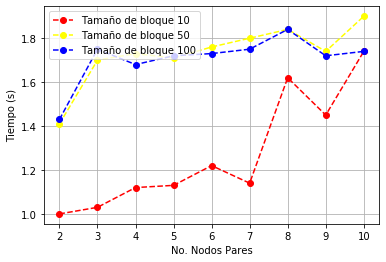
\includegraphics[scale=0.5]{Graphics/ComparacionLatencia10TPS.png}
\caption{Latencia promedio en redes con distinto tama\~no de bloque para escenarios de 10 TPS.}
\label{ComparacionLatencia10TPS}
\end{figure}


\subsection{An\'alisis de rendimiento}

\begin{figure}[h]
\subfigure[Tama\~no de bloque igual 10.]{
\begin{minipage}[t]{0.30\linewidth}
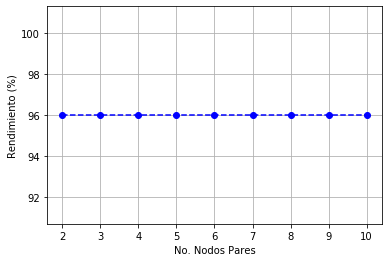
\includegraphics[scale=0.35]{Graphics/RendimientoPares10TPSBS10.png}
\end{minipage}
}
\subfigure[Tama\~no de bloque igual 50.]{
\begin{minipage}[t]{0.30\linewidth}
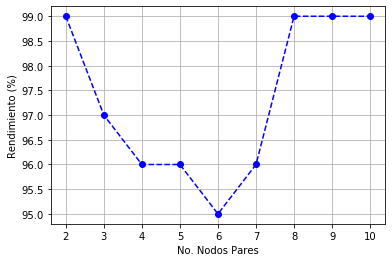
\includegraphics[scale=0.35]{Graphics/RendimientoPares10TPSBS50.png}
\end{minipage}
}
\subfigure[Tama\~no de bloque igual 100.]{
\begin{minipage}[t]{0.30\linewidth}
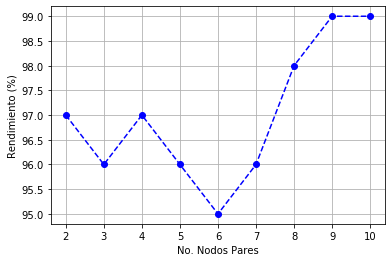
\includegraphics[scale=0.35]{Graphics/RendimientoPares10TPSBS100.png}
\end{minipage}
}
\caption{Rendimiento en distintas configuraciones de nodos pares en una red con un solo nodo ordenador para escenarios de 10 TPS.}
\end{figure}


Para los tama\~no de bloque planteados, los valores de rendimiento de la red oscilan entre el 95$\%$ y 99$\%$. La red configurada con tama\~no de bloque 10 mantiene un rendimiento constante de 96$\%$ para las configuraciones de nodos pares estudiadas.\\

 En el caso de la red con bloques de tama\~no 50 se alcanza un mejor rendimiento en la mayor\'ia de las configuraciones de nodos pares, como se puede ver en la figura \ref{RendimientoPares10TPS}.\\

\begin{figure}[h]
\centering
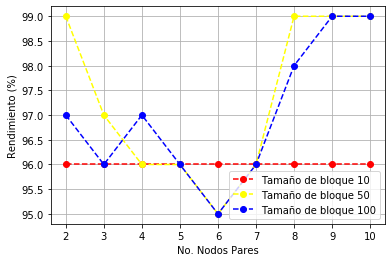
\includegraphics[scale=0.5]{Graphics/RendimientoPares10TPS.png}
\caption{Rendimiento de redes con distinto tama\~no de bloque para escenarios de 10 TPS.}
\label{RendimientoPares10TPS}
\end{figure}

\newpage

Para determinar una configuraci\'on \'optima, en relaci\'on a los valores de par\'ametros estudiados, se tuvo en cuenta el rendimiento en la red y la latencia promedio. Para establecer una comparaci\'on se llevaron las m\'etricas a una escala global, normalizando sus valores. Estos valores son estimaciones promedio para configuraciones con una cantidad de nodos pares entre dos y diez por organizaci\'on, donde el tama\~no en los bloques representa el factor a optimizar. En la figura \ref{Resultado10TPS} podemos ver que el mejor rendimiento se alcanza para canales con tama\~no de bloque igual a 50, pero a su vez la latencia promedio es mayor que la estimada para las configuraciones de canales de tama\~no 10. Por tanto, los valores 10 y 50 representan \'optimos locales, que en dependencia del escenario de uso, minimizan la latencia promedio y maximizan el rendimiento de la red respectivamente.\\

\begin{figure}[h]
\centering
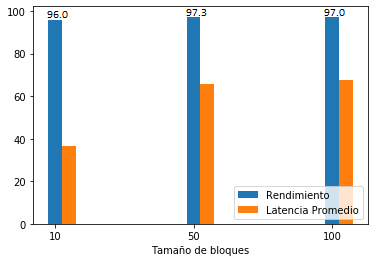
\includegraphics[scale=0.7]{Graphics/Resultado10TPS.png}
\caption{Evaluaci\'on de resultados para escenarios de 10 TPS.}
\label{Resultado10TPS}
\end{figure}

\newpage

\section{Escenario de alto volumen de transacciones}

En las tablas \ref{tab:100TPS-10BS}, \ref{tab:100TPS-50BS} y \ref{tab:100TPS-100BS} se registran los datos obtenidos para el escenario de 100 TPS.\\

\subsection{An\'alisis de latencia}

Las siguientes gr\'aficas muestran el comportamiento de la latencia promedio en la red configurada con cada tama\~no de bloque estudiado.\\

\begin{figure}[htbp]
\subfigure[Tama\~no de bloque igual 10.]{
\begin{minipage}[t]{0.30\linewidth}
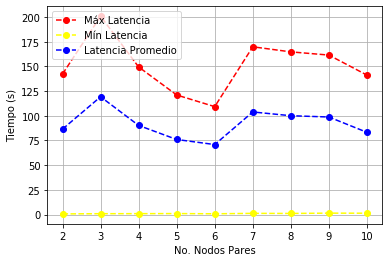
\includegraphics[scale=0.35]{Graphics/AnalisisLatenciaPares100TPSBS10.png}
\end{minipage}
}
\subfigure[Tama\~no de bloque igual 50.]{
\begin{minipage}[t]{0.30\linewidth}
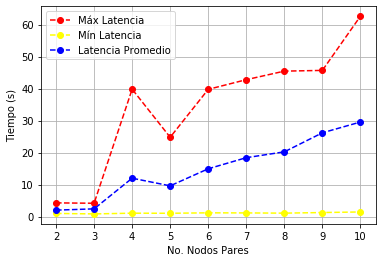
\includegraphics[scale=0.35]{Graphics/AnalisisLatenciaPares100TPSBS50.png}
\end{minipage}
}
\subfigure[Tama\~no de bloque igual 100.]{
\begin{minipage}[t]{0.30\linewidth}
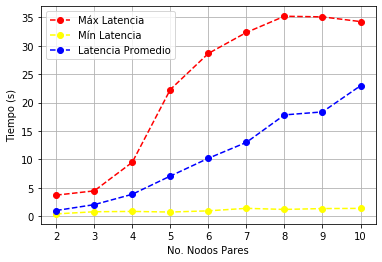
\includegraphics[scale=0.35]{Graphics/AnalisisLatenciaPares100TPSBS100.png}
\end{minipage}
}
\caption{Latencia en distintas configuraciones de nodos pares en una red con un solo nodo ordenador para escenarios de 100 TPS.}
\end{figure}


En la primera gr\'afica podemos observar que los valores de latencia promedio oscilan entre los 70 y 120 segundos aproximadamente. Estos valores son, en extremo, elevados en comparaci\'on con las restantes configuraciones. Para el caso de los bloques de tama\~no 100 el mayor valor alcanzado de latencia promedio, no supera los 25 segundos, quedando todos sus valores por debajo de los alcanzados por la configuraci\'on de bloques de tama\~no 10. Lo mismo sucede en las redes con bloques de tama\~no 50 que no superan los 30 segundos.\\

Para determinar el tama\~no de bloque que ofrece mejor desempe\~no en redes con un n\'umero de nodos pares que var\'ia de dos a diez por organizaci\'on,  con respecto a la latencia de las transacciones, se calcul\'o la media de las latencias promedios de las configuraciones de nodos pares, por tama\~nos de bloques, y nos quedamos con la configuraci\'on de bloque que corresponda a la menor de ellas.\\

Los bloques de tama\~no 10, 50 y 100 promedian una latencia media para las configuraciones de nodos pares de 92.1, 15.0 y 10.7 segundos respectivamente. Por tanto, las redes configuradas con bloques de tama\~no 100 son \'optimas respecto al conjunto estudiado, propiciando la menor latencia promedio. Para establecer una comparativa visual nos podemos remitir a la figura \ref{ComparacionLatencia100TPS}.\\

\begin{figure}[h]
\centering
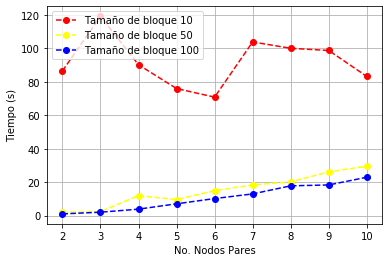
\includegraphics[scale=0.5]{Graphics/ComparacionLatencia100TPS.png}
\caption{Latencia promedio en redes con distinto tama\~no de bloque para escenarios de 100 TPS.}
\label{ComparacionLatencia100TPS}
\end{figure}

\subsection{An\'alisis de rendimiento}

\begin{figure}[h]
\subfigure[Tama\~no de bloque igual 10.]{
\begin{minipage}[t]{0.30\linewidth}
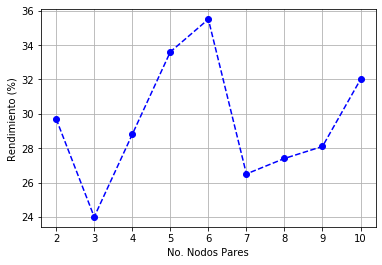
\includegraphics[scale=0.35]{Graphics/RendimientoPares100TPSBS10.png}
\end{minipage}
}
\subfigure[Tama\~no de bloque igual 50.]{
\begin{minipage}[t]{0.30\linewidth}
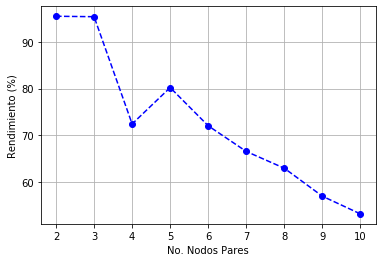
\includegraphics[scale=0.35]{Graphics/RendimientoPares100TPSBS50.png}
\end{minipage}
}
\subfigure[Tama\~no de bloque igual 100.]{
\begin{minipage}[t]{0.30\linewidth}
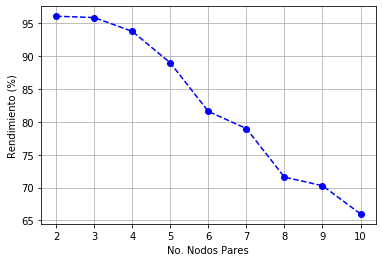
\includegraphics[scale=0.35]{Graphics/RendimientoPares100TPSBS100.png}
\end{minipage}
}
\caption{Rendimiento en distintas configuraciones de nodos pares en una red con un solo nodo ordenador para escenarios de 100 TPS.}
\end{figure}

De acuerdo a la gr\'afica que representa el rendimiento para las redes con bloques de tama\~no 10, se destaca el bajo rendimiento que logran en escenarios de altos vol\'umenes de transacciones. Entre las causas fundamentales que lo ocasionan est\'a el r\'apido llenado de los bloques por el servicio de ordenaci\'on, que luego son enviados, con mayor frecuencia, a los nodos pares para el proceso de validaci\'on y a su vez se conjuga con el alto volumen de transacciones que deben simular en cada intervalo de tiempo. Los bloques de tama\~no 50 y 100 manifiestan un mejor rendimiento debido a que compensan la frecuencia de validaci\'on por los nodos pares, con un aumento del tiempo de conformaci\'on de bloques.\\

Si ilustramos las curvas de rendimiento en una sola gr\'afica, como en la figura \ref{RendimientoPares100TPS}, apreciamos que las redes con bloques de tama\~no 100 superan para todas las configuraciones de nodos pares, a las redes con bloques de tama\~no inferior. Se aprecia adem\'as, que para escenarios de altos vol\'umenes de transacciones por segundo, el aumento del n\'umero de nodos pares en las organizaciones reducen el rendimiento de forma considerable.

\begin{figure}[h]
\centering
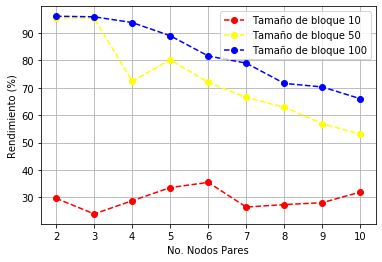
\includegraphics[scale=0.5]{Graphics/RendimientoPares100TPS.png}
\caption{Rendimiento de redes con distinto tama\~no de bloque para escenarios de 100 TPS.}
\label{RendimientoPares100TPS}
\end{figure}

En este escenario, la configuraci\'on para bloques de tama\~no 100, propicia la menor latencia promedio en la red y el mejor desempe\~no en el rendimiento, del conjunto evaluado. En la figura \ref{Resultado100TPS} se puede ver el marcado contraste dado por la diferencia en el tama\~no de los bloques. Se tiene una diferencia m\'axima de latencia superior a los 80 segundos, igual comportamiento tenemos en el rendimiento, donde los bloque de tama\~no 10 ofrecen las m\'etricas m\'as desfavorables. A su vez, esta coincide con la configuraci\'on, por defecto, de la red para los canales de comunicaci\'on. Por tanto, confirma la necesidad de evaluar los par\'ametros del sistema antes de su puesta en producci\'on.\\

\begin{figure}[h]
\centering
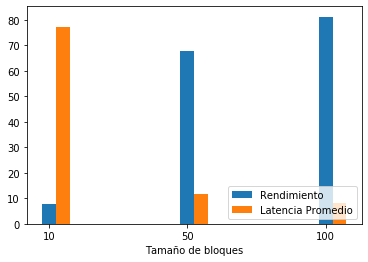
\includegraphics[scale=0.6]{Graphics/Resultado100TPS.png}
\caption{Evaluaci\'on de resultados para escenarios de 100 TPS.}
\label{Resultado100TPS}
\end{figure}

%\section*{An\'alisis de la influencia de los nodos pares y ordenadores en los escenarios estudiados}


\backmatter

\begin{conclusions}
    Conclusiones
\end{conclusions}

\begin{anexos}
 
\begin{table}[h]
\centering
\rowcolors{2}{gray!20}{}
\scalebox{0.7}{\begin{tabular}{ c  c }
\hline
Rango & Relaci\'on \\ 
\hline
\hline
-0.91 a -1.00 & Correlaci\'on negativa perfecta\\
-0.76 a -0.90 & Correlaci\'on negativa muy fuerte\\
-0.51 a -0.75 & Correlaci\'on negativa considerable\\
-0.11 a -0.50 & Correlaci\'on negativa media\\
-0.01 a -0.10 & Correlaci\'on negativa d\'ebil\\
0.00 No existe & Correlaci\'on\\
+0.01 a +0.10 & Correlaci\'on positiva d\'ebil\\
+0.11 a +0.50 & Correlaci\'on positiva media\\
+0.51 a +0.75 & Correlaci\'on positiva considerable\\
+0.76 a +0.90 & Correlaci\'on positiva muy fuerte\\
+0.91 a +1.00 & Correlaci\'on positiva perfecta\\
\hline
\end{tabular}}
\caption{Grado de relaci\'on seg\'un coeficiente de correlaci\'on. \emph{Fuente: Uso de la correlaci\'on de Spearman en un estudio de intervenci\'on en fisioterapia.}}
\label{tab:GradoCoeficiente}
\end{table} 
 
    
\begin{table}[h]
\centering
\rowcolors{2}{gray!20}{}
\scalebox{0.7}{\begin{tabular}{ c  c  c }
\hline
No. Organizaciones & No. Nodos Pares & No. Nodos Ordenadores/Nodos Kafka \\ 
\hline
\hline
1 & 2, 4, 8, 16 & 1 \\
2 & 2, 4, 8, 16 & 1 \\
4 & 4, 8, 16 & 1 \\
8 & 8 & 1 \\
2 & 2 & 2, 4, 8 \\
4 & 4 & 2, 4, 8 \\
\hline
\end{tabular}}
\caption{Configuraciones de la red. \emph{Fuente: Performance analysis of hyperledger fabric 2.0 blockchain platform.}}
\label{tab:Configuraciones}
\end{table}


\begin{table}[h]
\centering
\rowcolors{2}{gray!20}{}
\begin{tabular}{ c  c  c }
\hline
No. Nodos Pares & No. Nodos Ordenadores & Tama\~no de los bloques \\ 
\hline
\hline
2,3,4,5,6,7,8,9,10 & 1 & 10,50,100\\
\hline
\end{tabular}
\caption{Configuraciones de la red.}
\label{tab:MisConfiguraciones}
\end{table}



\begin{table}[h]
\centering
\rowcolors{2}{gray!20}{}
\scalebox{0.6}{\begin{tabular}{c  c  c  c  c  c  c}
\hline
No. Nodos Pares & No. Nodos Ordenadores & TPS & M\'ax. Latencia & M\'in. Latencia & Latencia Promedio & Rendimiento($\%$) \\ 
\hline
\hline
2 & 1 & 10 & 2.51 & 0.46 & 1.00 & 96.0 \\
3 & 1 & 10 & 2.60 & 0.52 & 1.03 & 96.0 \\
4 & 1 & 10 & 5.02 & 0.54 & 1.12 & 96.0 \\
5 & 1 & 10 & 4.49 & 0.56 & 1.13 & 96.0 \\
6 & 1 & 10 & 4.50 & 0.59 & 1.22 & 96.0 \\
7 & 1 & 10 & 4.46 & 0.53 & 1.14 & 96.0 \\
8 & 1 & 10 & 4.59 & 0.63 & 1.62 & 96.0 \\
9 & 1 & 10 & 4.87 & 0.60 & 1.45 & 96.0 \\
10 & 1 & 10 & 4.77 & 0.63 & 1.74 & 96.0 \\
\hline
\end{tabular}}
\caption{Evaluaci\'on escalando el n\'umero de nodos pares en una red con un tama\~no de bloque igual a 10 y un valor estimado de env\'io de 10 TPS.}
\label{tab:10TPS-10BS}
\end{table}


\begin{table}[h]
\centering
\rowcolors{2}{gray!20}{}
\scalebox{0.6}{\begin{tabular}{c  c  c  c  c  c  c}
\hline
No. Nodos Pares & No. Nodos Ordenadores & TPS & M\'ax. Latencia & M\'in. Latencia & Latencia Promedio & Rendimiento($\%$) \\ 
\hline
\hline
2 & 1 & 10 & 2.48 & 0.36 & 1.41 & 99.0 \\
3 & 1 & 10 & 2.86 & 0.57 & 1.70 & 97.0 \\
4 & 1 & 10 & 2.92 & 0.57 & 1.73 & 96.0 \\
5 & 1 & 10 & 4.74 & 0.56 & 1.71 & 96.0 \\
6 & 1 & 10 & 4.88 & 0.62 & 1.76 & 95.0 \\
7 & 1 & 10 & 5.03 & 0.65 & 1.80 & 96.0 \\
8 & 1 & 10 & 4.81 & 0.65 & 1.84 & 99.0 \\
9 & 1 & 10 & 4.68 & 0.53 & 1.74 & 99.0 \\
10 & 1 & 10 & 5.10 & 0.58 & 1.90 & 99.0 \\
\hline
\end{tabular}}
\caption{Evaluaci\'on escalando el n\'umero de nodos pares en una red con un tama\~no de bloque igual a 50 y un valor estimado de env\'io de 10 TPS.}
\label{tab:10TPS-50BS}
\end{table}


\begin{table}[h]
\centering
\rowcolors{2}{gray!20}{}
\scalebox{0.6}{\begin{tabular}{c  c  c  c  c  c  c}
\hline
No. Nodos Pares & No. Nodos Ordenadores & TPS & M\'ax. Latencia & M\'in. Latencia & Latencia Promedio & Rendimiento($\%$) \\ 
\hline
\hline
2 & 1 & 10 & 2.51 & 0.36 & 1.43 & 97.0 \\
3 & 1 & 10 & 3.13 & 0.63 & 1.75 & 96.0 \\
4 & 1 & 10 & 2.89 & 0.53 & 1.68 & 97.0 \\
5 & 1 & 10 & 2.81 & 0.61 & 1.72 & 96.0 \\
6 & 1 & 10 & 3.15 & 0.58 & 1.73 & 95.0 \\
7 & 1 & 10 & 3.05 & 0.60 & 1.75 & 96.0 \\
8 & 1 & 10 & 3.38 & 0.64 & 1.84 & 98.0 \\
9 & 1 & 10 & 2.98 & 0.59 & 1.72 & 99.0 \\
10 & 1 & 10 & 2.98 & 0.57 & 1.74 & 99.0 \\
\hline
\end{tabular}}
\caption{Evaluaci\'on escalando el n\'umero de nodos pares en una red con un tama\~no de bloque igual a 100 y un valor estimado de env\'io de 10 TPS.}
\label{tab:10TPS-100BS}
\end{table}


\begin{table}[h]
\centering
\rowcolors{2}{gray!20}{}
\scalebox{0.6}{\begin{tabular}{c  c  c  c  c  c  c}
\hline
No. Nodos Pares & No. Nodos Ordenadores & TPS & M\'ax. Latencia & M\'in. Latencia & Latencia Promedio & Rendimiento($\%$) \\ 
\hline
\hline
2 & 1 & 100 & 142.46 & 0.65 & 86.55 & 29.7 \\
3 & 1 & 100 & 200.83 & 0.88 & 119.27 & 24.0 \\
4 & 1 & 100 & 149.46 & 0.92 & 90.26 & 28.8 \\
5 & 1 & 100 & 121.09 & 1.01 & 76.02 & 33.6 \\
6 & 1 & 100 & 109.29 & 0.79 & 70.88 & 35.5 \\
7 & 1 & 100 & 169.89 & 1.21 & 103.89 & 26.5 \\
8 & 1 & 100 & 164.75 & 1.12 & 100.10 & 27.4 \\
9 & 1 & 100 & 161.51 & 1.43 & 98.79 & 28.1 \\
10 & 1 & 100 & 141.25 & 1.36 & 83.28 & 32.0 \\
\hline
\end{tabular}}
\caption{Evaluaci\'on escalando el n\'umero de nodos pares en una red con un tama\~no de bloque igual a 10 y un valor estimado de env\'io de 100 TPS.}
\label{tab:100TPS-10BS}
\end{table}


\begin{table}[h]
\centering
\rowcolors{2}{gray!20}{}
\scalebox{0.6}{\begin{tabular}{c  c  c  c  c  c  c}
\hline
No. Nodos Pares & No. Nodos Ordenadores & TPS & M\'ax. Latencia & M\'in. Latencia & Latencia Promedio & Rendimiento($\%$) \\ 
\hline
\hline
2 & 1 & 100 & 4.28 & 0.98 & 2.01 & 95.5 \\
3 & 1 & 100 & 4.16 & 0.83 & 2.41 & 95.4 \\
4 & 1 & 100 & 39.80 & 1.06 & 11.99 & 72.4 \\
5 & 1 & 100 & 24.78 & 1.03 & 9.60 & 80.2 \\
6 & 1 & 100 & 39.75 & 1.17 & 14.93 & 72.0 \\
7 & 1 & 100 & 42.77 & 1.14 & 18.40 & 66.5 \\
8 & 1 & 100 & 45.44 & 1.07 & 20.22 & 62.9 \\
9 & 1 & 100 & 45.67 & 1.26 & 26.17 & 56.9 \\
10 & 1 & 100 & 62.59 & 1.44 & 29.54 & 53.1 \\
\hline
\end{tabular}}
\caption{Evaluaci\'on escalando el n\'umero de nodos pares en una red con un tama\~no de bloque igual a 50 y un valor estimado de env\'io de 100 TPS.}
\label{tab:100TPS-50BS}
\end{table}


\begin{table}[h]
\centering
\rowcolors{2}{gray!20}{}
\scalebox{0.6}{\begin{tabular}{c  c  c  c  c  c  c}
\hline
No. Nodos Pares & No. Nodos Ordenadores & TPS & M\'ax. Latencia & M\'in. Latencia & Latencia Promedio & Rendimiento($\%$) \\ 
\hline
\hline
2 & 1 & 100 & 3.73 & 0.43 & 1.03 & 96.1 \\
3 & 1 & 100 & 4.48 & 0.81 & 2.06 & 95.9 \\
4 & 1 & 100 & 9.50 & 0.87 & 3.88 & 93.8 \\
5 & 1 & 100 & 22.29 & 0.76 & 7.08 & 89.0 \\
6 & 1 & 100 & 28.63 & 0.97 & 10.21 & 81.6 \\
7 & 1 & 100 & 32.32 & 1.41 & 13.00 & 79.0 \\
8 & 1 & 100 & 35.17 & 1.22 & 17.83 & 71.6 \\
9 & 1 & 100 & 35.06 & 1.37 & 18.36 & 70.3 \\
10 & 1 & 100 & 34.23 & 1.40 & 22.96 & 66.0 \\
\hline
\end{tabular}}
\caption{Evaluaci\'on escalando el n\'umero de nodos pares en una red con un tama\~no de bloque igual a 100 y un valor estimado de env\'io de 100 TPS.}
\label{tab:100TPS-100BS}
\end{table}

\end{anexos}

\begin{recomendations}
El estudio se realiz\'o sobre una muestra de par\'ametros de configuraci\'on, y se determin\'o con respecto a ellos, los que optimizan escenarios de 10 y 100 transacciones por segundo. Propongo extender la investigaci\'on para una muestra de tama\~no mayor, que permita realizar un an\'alisis en pruebas de hip\'otesis para tratar de obtener una generaliaci\'on en el comportamiento de la variaci\'on de los par\'ametros.\\

Determinar un tama\~no adecuado de los bloques en un canal de comunicaci\'on, resulta una tarea compleja producto a la influencia directa que tiene sobre varias de las componentes de fabric, como los nodos pares y los nodos ordenadores. Por lo que trabajar en una herramienta que itere de manera eficiente para converger hacia un posible candidato a tama\~no \'optimo ayudar\'ia en gran medida a encontrar los valores que mejoren el rendimiento en un escenario determinado.
\end{recomendations}

\printbibliography[heading=bibintoc]



\end{document}
